\documentclass[letterpaper]{sig-alternate-05-2015}

\usepackage{graphicx}
\usepackage{subfigure}
\usepackage{epsfig}
\usepackage{epstopdf}
\graphicspath{.}

\usepackage{appendix}

% use this package if you need more space
\usepackage{times}

\usepackage{relsize}
\usepackage{verbatim}
\usepackage{color}
\usepackage{paralist}
\usepackage{tabularx}
\usepackage{amssymb}
\usepackage{bbm}
\usepackage{ifthen}

% Math
\usepackage{amsmath}
\usepackage{mathtools}
\newcommand{\pluseq}{\mathrel{+}=}
\newcommand{\asteq}{\mathrel{*}=}
\DeclareMathOperator*{\argmin}{arg\,min}
\DeclareMathOperator*{\argmax}{arg\,max}

% Theorem, Lemma, etc.
\usepackage[capitalise]{cleveref}
\newtheorem{theorem}{Theorem}[section]
\newtheorem{definition}{Definition}
\newtheorem{lemma}{Lemma}
\newtheorem{proposition}{Proposition}
\newtheorem{corollary}{Corollary}
\newtheorem{example}{Example}

% Algorithms
\usepackage{algorithm}
\usepackage{algorithmic}
\renewcommand{\algorithmicrequire}{\textbf{Input:}}
\renewcommand{\algorithmicensure}{\textbf{Output:}}

% Floats
\usepackage{float}
\renewcommand{\textfraction}{0.00}
\renewcommand{\topfraction}{1.0}
\renewcommand{\bottomfraction}{1.0}
\setcounter{totalnumber}{100}
\setcounter{bottomnumber}{100}
\setcounter{topnumber}{100} 

% URLs
\usepackage{url}

% 
\usepackage{multirow}
\usepackage{colortbl}
\definecolor{kugray5}{RGB}{224,224,224}

% Captions
\usepackage{caption}
%\setlength{\belowcaptionskip}{-5pt}
%\setlength{\abovecaptionskip}{-1pt}
\captionsetup{font=bf}
\usepackage[justification=centering]{caption}

% Single/Double Qoutes
\newcommand{\qoute}[1]{`#1'}
\newcommand{\qoutes}[1]{``#1''}
\newcommand{\itqoutes}[1]{\textit{``#1''}}

\newcommand{\TODO}[2]{\textbf{\textcolor{red}{TODO: (#1) #2}}}
\newcommand{\dingedit}[1]{\textcolor{red}{\emph{[Ding: #1]}}}
\newcommand{\moedit}[1]{\textcolor{cyan}{\emph{[Mohammad: #1]}}}
\newcommand{\fname}{APART }

\title{Price-aware Real-time Ride-sharing at Scale -\\An Auction-based Approach}

\author{{Mohammad Asghari, Dingxiong Deng, Cyrus Shahabi, Ugur Demiryurek, Yaguang Li}\\
\fontsize{10}{10}\selectfont\rmfamily\itshape
University of Southern California, Los Angeles, CA, USA\\
\fontsize{9}{9}\selectfont\ttfamily\upshape
\{masghari,dingxiod,shahabi,demiryur,yaguang\}@usc.edu\\
}

\begin{document}

\CopyrightYear{2016} 
\setcopyright{acmcopyright}
\conferenceinfo{SIGSPATIAL'16,}{October 31-November 03, 2016, Burlingame, CA, USA}
\isbn{978-1-4503-4589-7/16/10}\acmPrice{\$15.00}
\doi{http://dx.doi.org/10.1145/2996913.2996974}

\maketitle

\begin{abstract}
Real-time ride-sharing, which enables on-the-fly matching between riders and drivers (even en-route), is an important problem due to its environmental and societal benefits. With the emergence of many ride-sharing platforms (e.g., Uber and Lyft), the design of a scalable framework to match riders and drivers based on their various constraints while maximizing the overall profit of the platform becomes a distinguishing business strategy.\\
A key challenge of such framework is to satisfy both types of the users in the system, e.g., reducing both riders' and drivers' travel distances. However, the majority of the existing approaches focus only on minimizing the total travel distance of drivers which is not always equivalent to shorter trips for riders. Hence, we propose a fair pricing model that simultaneously satisfies both the riders' and drivers' constraints and desires (formulated as their profiles). In particular, we introduce a distributed auction-based framework where each driver's mobile app automatically bids on every nearby request taking into account many factors such as both the driver's and the riders' profiles, their itineraries, the pricing model, and the current number of riders in the vehicle.  Subsequently, the server determines the highest bidder and assigns the rider to that driver. We show that this framework is scalable and efficient, processing hundreds of tasks per second in the presence of thousands of drivers. We compare our framework with the state-of-the-art approaches in both industry and academia through experiments on New York City's taxi dataset.  Our results show that our framework can simultaneously match more riders to drivers (i.e., higher service rate) by engaging the drivers more effectively. Moreover, our framework schedules shorter trips for riders (i.e., better service quality). Finally, as a consequence of higher service rate and shorter trips, our framework increases the overall profit of the ride-sharing platforms.
\end{abstract}

\vspace{-0.15in}
\section*{Categories and Subject Descriptors}
\vspace{-0.025in}
H.3.5 [\textbf{Information Storage and Retrieval}]: Online Information Services-\textit{Commercial services}

\vspace{-0.1in}
\section*{Keywords}
\vspace{-0.025in}
Ride-sharing, Revenue Maximization, Spatial Crowdsourcing

\section{Introduction}
\label{sec:intro}
%TO-DO lists:
%\begin{itemize}
%	\item Problem definition: define driver profile, rider profile and our price model.
%	
%	\item Define our objective functions (i.e., maximize extra profit), and differentiate it with other optimization goal (e.g., minimize extra distance). 
%	%Given a rider and a driver with their profiles, calculate the cost of accepting the rider. 
%	
%	\item Introduce overall framework, and describe our auction-based mechanism.
%	
%	\item Properties of our framework in both local setting and global setting. In the local setting, show that we will get the same profit as the centralized setting. In the global setting, show that our technique can achieve certain approximation ratio compared with the global optimal (or upper bound of global optimal),  or vice verse we will suffer from certain degenerated cases.
%	
%	\item Optimizations: a) Maintain coarse-grained hierarchic index (adaptive grids, quad-tree), b) maintain novel shortest path index which is fine tuned for ride-sharing applications c) batch processing rider requests (single round bidding v.s. multi-round bidding).
%	
%\end{itemize}

%%%%%% 1. background information
% Ridesharing becomes popular recently because it has potential to match riders with similar itineraries and time schedules, and to bring significant benefits to individual users and the city as a whole. 

Real-time ride-sharing, as an alternative transportation service, alleviates traffic congestion and decreases auto emissions. With the emergence of many commercial platforms (e.g., Uber and Lyft), which automatically match drivers and riders on-the-fly, real-time ride-sharing becomes more and more popular. According to~\cite{uberpool}, millions of trips have been taken on UberPool since its launch at August 2014, and thousands of passengers take it five times a week during commuting hours. Enabled by the development and technology advances of smart phones and location-based services, ride-sharing platforms typically operate as follows: (1) Riders and drivers can join the platform via their smart phones, (2) a rider can submit a request, which consists of the pick-up and drop-off points, to the platform, (3) once a new request is received, the platform determines a driver (even en-route) to pick up the rider, (4) when the trip is completed, the platform calculates the rider's fare and the driver's income. With these platforms, riders can share a vehicle with reduced trip cost while enjoying fast and convenient transportation.

%%%%%% 2. explain the challengs and the detour of ridesharing......
Many challenges exist to enable such real-time ride-sharing platforms. From a business point of view, the platform provider (e.g., Uber) seeks to maximize its own profit. However, higher profits should not be at the cost of either charging passengers more or paying drivers less than what would compromise participation and retention due to no monetarily incentive for either parties. Consequently, the design of a fair pricing model becomes an essential business strategy. This is particularly important in cases of carpooling where riders share their ride with other riders. Even though carpooling reduces the riders' cost, it incurs extra distance (i.e., detour) for riders. While each rider's fare should be discounted as a function of the length of the detour, the driver should be rewarded more as the total travel distance is increased due to all detours. Furthermore, different users (i.e., riders and drivers) might value their time differently. Therefore, a fair pricing model should be available to both riders and drivers to express, for a certain amount of detour, how much discount or compensation they expect. Finally, in addition to fair pricing scheme for riders and drivers, the model should account for the provider's revenue as well.

The second challenge of a ride-sharing platform is to process incoming requests in real-time. This involves two different tasks: i) checking which drivers can add the new requests (new pick-up and drop-off locations) to their current trip without violating the constraints of that trip (i.e., scheduling) and ii) selecting the best driver among those who can serve the new request (i.e., matching). Processing the schedule of potentially thousands of drivers to check if they can accommodate a new request, with the additional task of matching their pricing profile with the incoming rider's profile, becomes computationally intensive. Therefore, the design of an efficient and scalable algorithm that assigns riders to drivers with a fair pricing model while maximizing the provider's revenue, is very challenging.


%First, the framework should consider the conflicting interests of different users (i.e., riders and drivers) and platform providers (e.g., Uber). For example, riders would like to arrive at their destination as quick and cheap as possible, whereas drivers and platform providers would like to maximize their profits. Although ride-sharing can reduce the cost of riders by sharing similar itineraries, it also incurs extra travel distance (i.e., detour). Ideally, riders are expected to be compensated for their detour, while drivers are expected to earn more profit. These factors makes the design of a fair pricing scheme (i.e., the fares and incomes) that satisfies the requirements of both riders and drivers even more complex. Secondly, because the riders requests are generated on-the-fly, the framework should decide the matching drivers (even en-route) at a short amount of time. Therefore, the design of an efficient framework that match riders and drivers, with a fair pricing scheme that provides incentives for all participants becomes a distinguishing business strategy. 

%%% 3. show the shortcomings of existing work and how they fail to address the challenge
The majority of previous studies~\cite{Ota15, Cici15, Cao15, PelzerITS15} focus on improving the efficiency of on-the-fly assignment with the objective of minimizing the total travel distance of drivers. In particular, in existing studies a new request is assigned to a driver who can fit the request in his schedule with the least amount of increase in the total traveled distance. However, minimizing drivers' total travel distance is not always equivalent to overall shorter trips for riders. Consequently, when assigning a new request, the driver who would incur the minimum increase in total travel distance is not necessarily the most cost effective option. To illustrate, suppose driver $a$ has two passengers on board and driver $b$ has only one. To serve an incoming request, \textit{a}'s incurred detour is 2 miles while for $b$ the detour is 3 miles. Even though $a$'s detour is shorter, the platform owner has to compensate both passengers of $a$ for 2 miles (a total of 4 miles) while in the case of $b$ it has to compensate only one passenger for a total of $3$ miles. In addition, from the riders' perspectives, in the first scenario two riders incur extra detour while in the second only one rider incurs an extra detour.  Few studies~\cite{Ma13,Ma15} consider a pricing model by defining monetary incentives for riders and drivers. In \cite{Ma13}, a pricing model is introduced where instead of being compensated, a rider can potentially end up being penalized for longer detours by paying a higher fare. Ma et. al.~\cite{Ma15} overcomes the unfairness issue in \cite{Ma13} to some extent. Even though, a new rider can incur detour in his trip, their model only compensates riders that are already on board. In addition, since this model is targeted for a different application, the notion of revenue fails to provide any incentive for the platform provider. Furthermore, in all previous studies~\cite{Ma13,Huang14,Ma15}, a centralized server is responsible for matching and scheduling incoming requests. Most of these studies utilize a spatiotemporal index to enable matching, i.e., narrowing down the number of potential drivers who can serve an incoming request. With thousands of drivers in the system, even after applying the spatial index, the centralized server still needs to perform scheduling and profile matching for all the candidate drivers. We show that with large number of drivers, these frameworks fail to process new requests in real-time (\cref{subsec:exprp}) and hence not scalable.


%in In \cite{Ma13}, a pricing model is introduced where instead of being compensated, a rider can potentially end up being penalized for longer detours by paying a higher fare. 

%In a recent study \cite{Ma15}, the pricing model overcomes the unfairness issue in \cite{Ma13} to some extent. Since riders can value their time differently, It also allows riders to accept/reject ride-sharing requests based on the amount they will be compensated for the incurred detour. However, drivers can similarly value their time different from each other. The pricing model in \cite{Ma15} does not provide any means for drivers to specify their monetary expectations for participating in the system. Furthermore, since this model only tends to divide the cost of the ride among riders, the notion of revenue is left out and it does not provide any incentive for the platform provider.


%%% 4. explain our pricing model, and provide more intuition of better service quality.
To address aforementioned challenges, in this paper, we introduce an Auction-based Price-Aware Real-time (\textit{APART}) ride-sharing framework. We propose a general and versatile pricing model that allows both riders and drivers to set their monetary expectations for participating in ride-sharing based on their predefined profiles. Specifically, each rider's profile defines the expected discount ratio for the detours incurred by ride-sharing. For example, one rider can express that he is willing to accept a 10 mile detour for 30\% discount. On the other hand, each driver's profile defines the expected cost in terms of his total travel distance and time. The model also accounts for the revenue of the platform provider. Consequently, our objective is to maximize the revenue of the ride-sharing framework while satisfying various temporal and monetary constraints of all users. APART is price-aware because a new request is assigned to a driver which generates the highest profit. Since our pricing model is designed to compensate riders for detours, the most profitable choice is also the one where \textit{riders} incur the least amount of detour, hence better service quality. Finally, APART also maximizes the revenue of the provider by increasing the service rate (throughput) in the system through engaging available drivers more effectively to serve more requests.


% With our price scheme, our objective is to maximize the total profit of the ridesharing platform, while satisfying the constraints of both riders and drivers.

% Because our pricing model compensates riders for longer trips, in order to maximize the profit, our framework reduces the detour of passengers and hence, providing better service quality. 

%We define a fair price model, which is flexible and general. The profiles are served to xxx. The constraints of are expressed as profiles. Given a user and rider profile, the fare and cost of xxx can be automatically derived from their profiles and other constrains. 

%%% 5. explain our framework
To efficiently assign riders to the candidate drivers, we introduce a distributed auction-based framework. With our framework, APART, the server broadcasts a new request to a set of candidate drivers and the mobile app of each candidate driver\footnote{Hereafter we use the term \qoutes{driver} to refer to both the human driver and the software running on his mobile device.} computes and submits a bid based on the driver's current schedule, his and his other passengers' profiles and other spatiotemporal constraints. Subsequently, the server collects all the bids from candidate drivers and assigns the rider to the highest bidding driver. To guarantee high service quality, each driver runs a branch-and-bound algorithm that performs an exhaustive search to find out whether it can fit a new request into its current scheduling. Each driver carries a small number of riders so even an exhaustive search can be performed in real-time. Due to the distributed nature of APART, all candidate drivers perform the search in parallel. Once each driver finds its own best schedule, the server simply selects the driver that generates the highest profit. Consequently, APART is able to find the most profitable drivers in real-time.


%With APART, the server does not need to know the exact location of every driver as it is not responsible for performing the scheduling phase. The grid index structure in APART, only needs to store which grid cell a driver is located in. Therefore, compared to a spatial index structure where the exact location of every driver is stored, APART's grid index requires fewer updates and less maintenance, which further reduces the load on the server.

%%% 6. show some experiment resutls

We conducted extensive experiments on a large scale New York City taxi dataset and show that APART is scalable and efficient, capable of processing hundreds of tasks per second in the presence of thousands of drivers. By comparing our framework with the state-of-the-art approaches~\cite{Huang14}, we show that our framework can simultaneously match up to 10\% more riders to drivers (i.e. higher service rate), while the total travel distance of riders are 20\% less (i.e., better service quality), hence our framework can generate more profit than other approaches with an even better service quality. On the other hand, we show that in a framework were riders are assigned to drivers with the least increase in the driver's travel distance, up to 25\% of the requests are not assigned to the most profitable driver. 

The remainder of this paper is organized as follows. We define our problem in \cref{sec:problem_def}, and explain our pricing model in \cref{sec:pricing}. We present our APART framework, and discuss its auction-based approach in \cref{sec:framework}. In \cref{sec:exp}, we report the experiment results. We discuss the related work in \cref{sec:related} and conclude the paper in \cref{sec:conclusion}.


%%%%%%%%%%%%%%%%%%%%%%%%%%%%%%%%%%%%%%%%%%%%%%%%%%%%
%%% from mohammod 

% Because platforms like Uber and Lyft are becoming more popular (we can show some numbers how their businesses are growing in the recent years). Ridesharing become popular recently. Existing ridesharing studies mainly focus on matching riders and drivers only considering their spatiotemporal constraints (max wait time, maximum detour, etc.)

% It is important to design systems that not only satisfy spatiotemporal constraints of the users, but also take into consideration the monetary aspect of the business (i.e., the fees riders pay, the drivers' income and the system's profit). A key component of such framework is to xxx and xxx.

% While most studies ignore this aspect of the system, T-Share provides a pricing model where on average riders end up paying less when compared to each passenger riding alone. However, based on some experimental results on NYC's taxi dataset, we noticed based on this pricing model, up to x\% of passengers end up paying even more that what they would have payed if they did not share a ride. Hence, this requires the design of a pricing model which is fair to every passenger meaning that if a passenger's trip gets longer as a result of sharing a ride, they should end up paying less (receiving a discount).

% To address the above challenges, in this paper we propose xxx. The goal of our framework is to maximize the profit of the platform. Because we utilize a pricing model which compensates riders for longer trips, in order to maximize the profit, our framework reduces the detour of passengers and hence, providing better service quality.

% Also, APART utilized an auction based approach allowing it to scale by distributing the computation among drivers (You can probably use a good chunk of this part from my CIKM submission).

% We evaluated our .

% The paper is organized as follows:

\section{Problem Definition}

In this section, we define the terminologies and a generic pricing model used in the paper.  At the end we give a formal definition of the problem under consideration.
%Next we define rider request, driver, price models (user and rider profiles), and our optimization goals.

\subsection{Basic Concepts}
The road network is represented as a graph $G(V, E)$, where each node represents intersections, and each edge represents a road segment. 
Each edge $(u,v) \in E$ $(u, v \in V)$ is associated with a weight $c(u,v)$ which is a travel cost (can be time or distance) from $u$ to $v$.
% TODO: define path in road network
The shortest path cost $d(s,t)$ is defined as the minimal cost paths connecting $s$ and $t$. In this paper, time and distance can be converted from one to the other.

\begin{definition} [Ride Request]
\label{def:req}
A ride request r can be represented as $\left\langle s, e, w, f \right\rangle$ consisting of a starting point $s \in V$ and an end point $e \in V$. Each request also specifies $w$ as the maximum time the rider can wait after making a request. In addition, a rider's profile $f: \delta d \rightarrow \left[ 0, 1 \right] $, specifies the relative discount in exchange for an incurred detour of $\delta d$.
%the ridesharing fare she would accept based on the extra detour and the shortest possible trip.
\end{definition}

Upon the acceptance of a request, \fname assigns it to a driver.

\begin{definition} [Driver]
A driver v is a human, driving a vehicle on the road network and is represented as $\left\langle TR, n, g \right\rangle$ where $TR$ is the list of v's assigned ride requests and $n$ is the maximum number of requests v can accept at any point in time. A driver also has a profile $g: d \rightarrow \$ $ which specifies the monetary cost of v driving a distance d while servicing its assigned requests.
\end{definition} 

\begin{definition} [Schedule]
Given a set $TR$ with n requests, a schedule $s= \left\langle x_1, \cdots, x_{2n} \right\rangle$ is an ordered sequence of pickup and delivery points for these request, where for each $r_i \in TR$, $r_i.s$ preceds $r_i.e$ in $s$. 
\end{definition}

A schedule is \textit{valid} for driver \textit{v}, if it satisfies the following conditions:

\begin{itemize}
\item waiting time constraint
\item capacity constraint
\item profit constraint, which is the price constraint based on rider and driver profiles. \moedit{need a more formal definition for this}
\end{itemize}

The driver will follow the sequence of picking up and dropping off riders. The schedule changes over time as riders are picked-up/dropped-off and new requests are added to the schedule. In fact, adding a new request to a schedule, may re-order some of the request that already exist in the schedule.

\begin{definition} [Matching]
Assuming we have a set of Drivers V and a set of Requests R, we call $M \subset V \times R$ a matching if for each $r \in R$ there is at most one $v \in V$ such that $\left( v, r \right) \in M$. We call $\left( v, r \right) \in M$ a \emph{match} and say $r$ has been matched to $v$.
\end{definition}

\noindent In a matching $M$, for every driver $v$, there exists a valid schedule $s_v$, such that $(v, r_i) \in M \implies r_i.s \in s_v \wedge r_i.e \in s_v$ (or simply $r_i \in s_v$). 

\subsection{Pricing Model}

Following the definition of basic concepts in the ride sharing system, we introduce a general price model that can be utilized to compute the corresponding fare of a ride, the payment drivers receive and subsequently, the profit the ride sharing system generates. Before we continue, it is necessary to point out that one of the building blocks of any real-world ride sharing system is a mechanism for computing the shortest path between any two points in the road network. Without loss of generality, we define our pricing model based on a static shortest path computations as opposed to time-dependent. However, the definitions can be easily updated to be compatible with time-dependent networks as well. For example, the fare of a ride is dependent on the distance between the pick-up and the drop-off points in a static network where in a time-dependent network it can be dependent on the travel time between those two points or perhaps both distance and travel time.

Every request $r$ has a default fare based on the shortest distance, $d_r$, from $r.s$ to $r.e$. In other words, we have an arbitrary function $FARE: d \rightarrow \$ $ such that $FARE(d)$ is the default fare of a ride. In a ride sharing system, the actual route between the pick-up and drop-off locations of a ride is not necessary the shortest route between the two points. We show the actual route between the two end points of a ride with $d'_r$ and define the detour of a ride as $\delta d_r = d'_r - d_r$. As explained in \cref{def:req}, each request is associated with a profile. We introduce the concept of a \textit{rider's profile} as a tool for the rider to specify how much discount she expects to receive in return for a certain amount of detour on her trip. A rider's profile can have different formats: linear decay, exponential decay, etc. \cref{fig:rider_profile} shows an example of a rider's profile.

\begin{figure}[!ht]
	\centering
	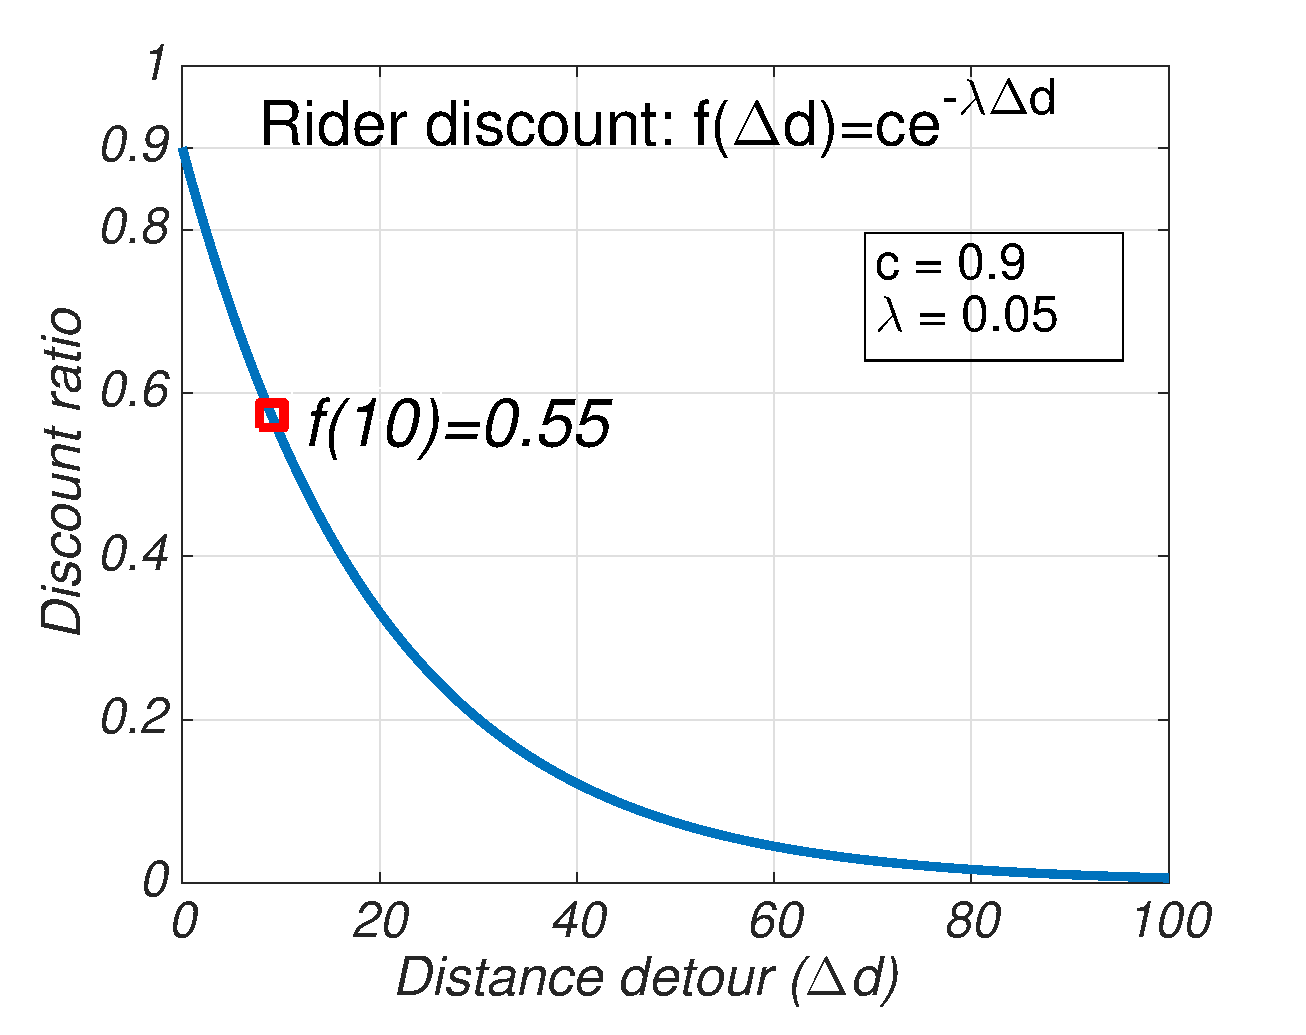
\includegraphics[width = 60mm]{fig/rider.eps}
	\vspace{-0mm}\caption{Rider profile} \vspace{-2mm} \label{fig:rider_profile}
\end{figure}\vspace{-0mm}

Subsequently, for a request $r$ with shortest distance $d_r$, detour $\delta d_r$ and a profile $f_r$, the final fare is $fare(r) = F(d_r) f_r(\delta d_r)$.

Every driver has a unique profile which allows him to specify the cost of his service. Similar to a rider, a driver's profile can be any function. In fact, the function can take any arbitrary input in addition to the distance. For example, it is possible to define the driver's profile as $g: n, d \rightarrow \$$ where $n$ is the number of passengers being serviced by the driver. Without loss of generality, in this paper we assume distance is the only input of the profile. Intuitively, the profile is a monotonically increasing function. For example, the profile in \cref{fig:driver_profile} is one where the driver charges \$1 per mile.

\begin{figure}[!ht]
	\centering
	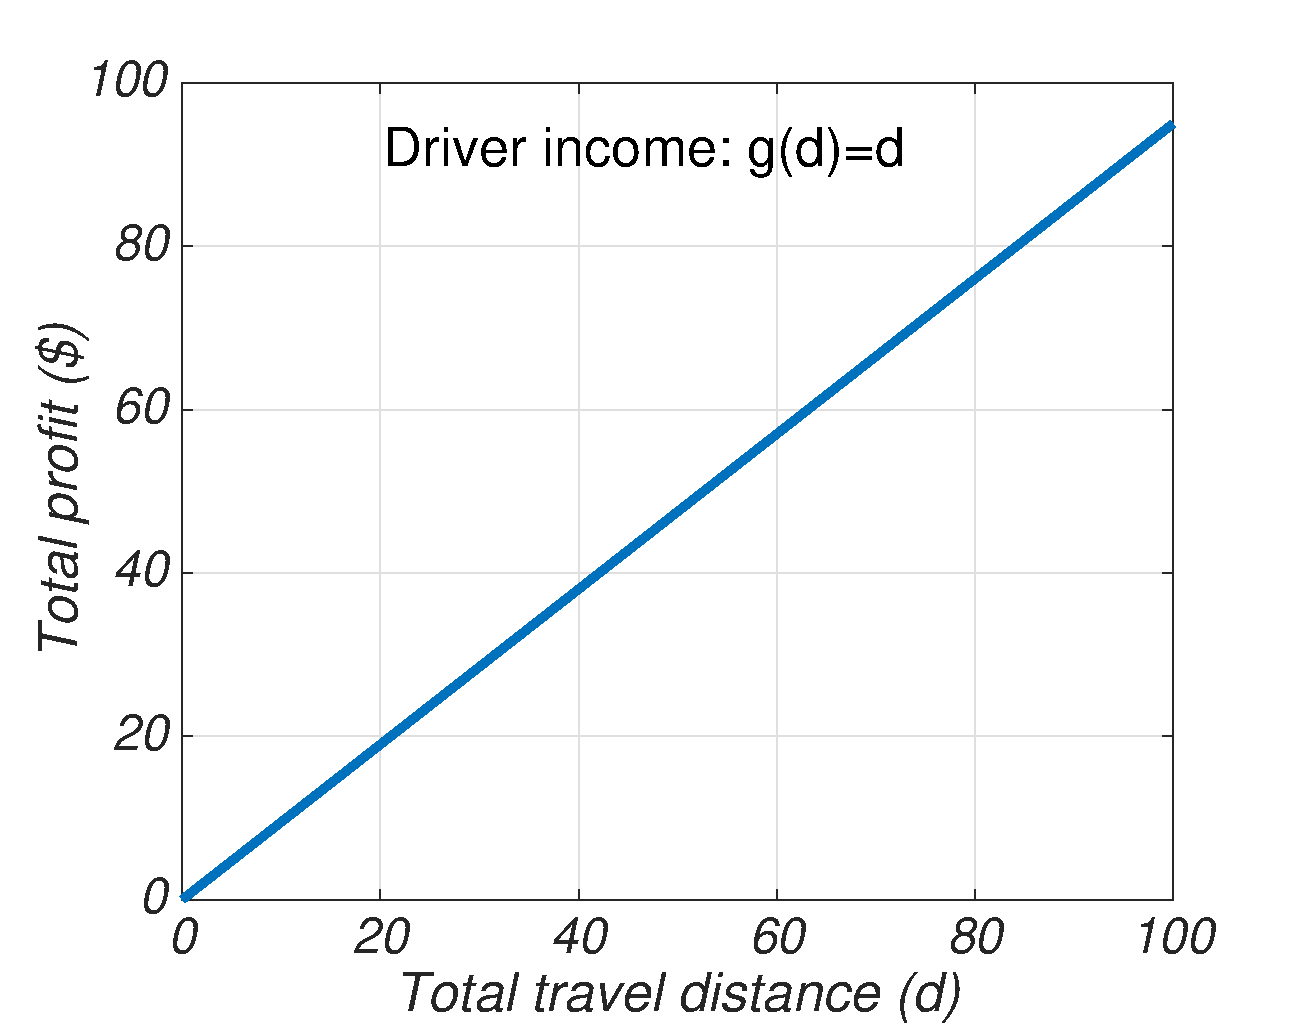
\includegraphics[width = 60mm]{fig/driver.eps}
	\vspace{-0mm}\caption{Driver profile} \vspace{-2mm} \label{fig:driver_profile}
\end{figure}\vspace{-0mm}
 
At any point in time, each driver has a schedule. A driver will be compensated during the time its schedule is not empty. Therefore, for every driver $v$, the payment he receives is:

\begin{equation*}
payment_v = \int_{start_s}^{end_s} I\left( s_v(t) \neq \left\langle \right\rangle\right).g(dist(t))dt
\end{equation*}

\noindent Where $I()$ is the indicator function, $s_v(t)$ and $dist(t)$ are the driver's schedule and the distance he travels at time $t$ respectively. In addition, $start_s$ and $end_s$ are the first pick-up time and last drop-off time of $s_v$.

The profit \fname makes from driver $v$ is the difference between the fares collected from all requests serviced by $v$ and the payment $v$ receives for himself. Subsequently, the total profit (revenue) of the system will be the sum of the profits received from all drivers:

\begin{align*}
profit_v &= \sum_{r_i \in s_v}fare(r_i) - payment_v\\
revenue &= \sum_{v \in V}profit_v
\end{align*}

Now that we have defined a generic pricing model, we can define the \textit{Ride-Sharing} problem as follows:

\begin{definition} [Ride-Sharing Problem]
Given a set of ride requests R and a set of drivers V, the goal of the Ride-Sharing problem is to find a matching M between R and V such that the revenue of M is maximized.
\end{definition}

\dingedit{Justify that our objective function is different with minimizing the travel cost.} \moedit{If we have space at the end, we can give a simple contrary example to prove this.}

%%% TODO: given a rider and the current schedule, calculate the extra profit of inserting a new request.


%Properties of the above definition, can we guarantee the extra profit should be positive?


\section{Pricing Model}
\label{sec:pricing}
%\section{System Overview}

\begin{enumerate}
\item What is a good profile for the rider?
\item What is a good profile for the driver?
\item How should a driver compute its bid?
\item How should the server select a winner?
\item What is a good optimization goal?
\end{enumerate}
\vspace{-4mm}
\section{APART Framework}
\vspace{-1mm}
\label{sec:framework}

In a real-time ride-sharing application, once the server receives a request, it needs to determine the driver who can best accommodate the new request with respect to his current schedule. With a large number of candidate drivers, the scheduling phase becomes the bottleneck in centralized frameworks where one single server processes the requests. Therefore, we introduce APART which overcomes this shortcoming by distributing the scheduling task to the drivers themselves. We first explain the auction framework in which the server broadcasts new arriving requests to the drivers. Subsequently, we discuss how each driver generates a bid based on its current schedule.

\subsection{Dispatch Requests}
\label{subsec:dispatch}
Auction frameworks have been effectively used for assignment problems \cite{Lagoudakis04,Mehta05}. Following the terminology used in auction frameworks, APART considers drivers as bidders and ride requests as goods. Note that the actual human driver does not engage in bidding, instead, his mobile app software does the bidding based on various constraints and goals. The server plays the role of a central auctioneer in APART. With APART, once a new request is received by the server (auctioneer), it presents the request to the drivers (bidders). Each driver computes a new schedule which incorporates the incoming request, and generates a bid based on the driver's and riders' profile. Subsequently the bid is submitted to the server. The bidding process is performed as a \textit{sealed-bid auction} where drivers simultaneously submit bids and no other driver knows how much the other drivers have bid. In the end the server selects the driver with the highest bid as the winner and matches the request with the driver.

With APART, drivers that are far away from the pick-up location of an incoming request, are not asked to bid on the request. The server only sends an incoming request to \textit{eligible drivers} that are defined as:
%With APART, the server does not need to know the exact location of every driver as it is not responsible for performing the scheduling phase. Consequently, APART utilized a grid index which only keeps track of which grid cell a driver is located in. Therefore, compared to a centralized setting where the exact location of every driver is stored, APART's grid index requires fewer updates and less maintenance, which further reduces the load on the server.

\begin{definition} [Eligible Drivers]
An available driver $v$ is said to be eligible for servicing a newly submitted request $r$, if and only if:
\vspace{-2mm}
\begin{equation*}
distance(v, r.s) \leq r.w \times avg\_speed
\end{equation*}
\end{definition}

\vspace{-2mm}
\begin{figure}[!ht]
	\centering
	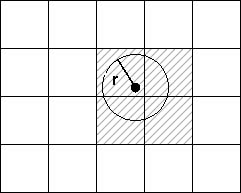
\includegraphics[width=0.65\columnwidth]{fig/grid_index}
	\vspace{-0mm}\caption{Spatiotemporal Grid Index} \vspace{-2mm} \label{fig:grid_index}
\end{figure}\vspace{-0mm}

\noindent In other words, an available driver \textit{d} is eligible for serving request \textit{r}, if he has enough time to reach the pick-up location of \textit{r} within \textit{r}'s waiting time. In order to find eligible workers for each request, the server maintains a spatial index on the location of the drivers. With APART, the server does not need to know the exact location of the drivers to filter out non-eligible drivers. We use a grid index where the server only keeps track of which cell a driver is located in. For example, in \cref{fig:grid_index}, assuming the black dot is the pick-up location of a new request and $r$ is the maximum wait time for the new request, any driver in the shaded cells will receive the new request. In our grid index, we use the filter and refine process in \cite{Demiryurek09} in order to enable continuous query processing on the underlying road network using Euclidean distances.

\begin{algorithm}
\caption{Dispatch($V_r, r, startTime$)}
\label{algo:dispatch}
\begin{algorithmic}[1]
\REQUIRE $V_r$ is the set of currently available drivers, $r$ is a new request and $startTime$ is the current time
\ENSURE $v \in V_r$ as the driver that request $r$ is assigned to
\STATE $v_{selected} \leftarrow $ \emph{null}
\STATE $Bids \leftarrow \emptyset$
\FOR{$v \in V_r$} \label{line:loop_start}
	\STATE $b_v \leftarrow $ ComputeBid$(v, v.schedule, r, startTime)$ \label{line:compute}
	\STATE $Bids \leftarrow Bids \cup \{b_v\}$
\ENDFOR \label{line:loop_end}
\STATE $v_{selected} \leftarrow \argmax_x \left\lbrace b_x \in Bids \right\rbrace$ \label{line:select}
\RETURN $v_{selected}$
\end{algorithmic}
\end{algorithm}
\vspace{-3mm}
\cref{algo:dispatch} outlines the process of assigning an incoming request $r$, where $V_r$ is the set of eligible drivers for request $r$ (line~\ref{line:loop_start}). For each candidate driver $v$, the \emph{ComputeBid} method (line \ref{line:compute}) is executed to perform scheduling and compute $v$'s bid (\cref{subsec:bidcomp}). Subsequently, the platform chooses the driver with the highest bid. In case of a tie in line \ref{line:select}, the algorithm randomly selects one driver among the ones with the highest bid. Notice that all the iterations of the \textbf{for} loop in \cref{algo:dispatch} (lines \ref{line:loop_start}-\ref{line:loop_end}) run in parallel.

\subsection{Bid Computation \& Payments}
\label{subsec:bidcomp}

Once a driver is notified of a new request, it has to compute a bid. The bid each driver generates reflects the profit the system can gain if the request is assigned to that driver. Once the ride-sharing application receives the request, it generates a bid and submits the bid to the server. When a new request is assigned to a diver, he will be notified with an updated schedule. This means that the human driver's interaction with APART is limited to configuring his profile on the ride-sharing application.

%\begin{algorithm}[!h]
%\caption{ComputeBid($v, r, time$)}
%\label{algo:comp_bid}
%\begin{algorithmic}[1]
%\REQUIRE $v$ is a driver, $r$ is a new request and $time$ is the current time.
%\ENSURE additional $profit$ that $v$ can generate by accepting $r$
%\STATE $src = \lbrace r'.s | r' \in v.schedule \rbrace$ 
%\STATE $src.$add$(r.s)$
%\STATE \small{$profit_n, schedule = $FindBestSchedule$(\emptyset, src, -\infty, \emptyset,  time)$} \label{ln:fbs}
%\STATE $profit_c, cost_c = $GetProfitAndCost$(v.schedule, time)$ \label{ln:gps}
%\RETURN $profit_n - profit_c$
%\end{algorithmic}
%\end{algorithm}
%
%\vspace{-.2in}
%
%\begin{algorithm}[!h]
%\caption{GetProfitAndCost($schedule, start$)}
%\label{algo:get_profit}
%\begin{algorithmic}[1]
%\REQUIRE \emph{schedule} is an ordered list of pick-up/drop-off points and \emph{start} is the current time.
%\ENSURE a pair of ($profit, cost$) of performing the input schedule. If the input schedule is not valid it returns ($-\infty, \infty$)
%\STATE $time = start$
%\STATE $loc = v.$loc\label{ln:loc}
%\STATE $trip = 0$
%\FOR{$p$ \textbf{in} $schedule$}
%	\STATE $path =$ ShortestPath($loc, p$.loc)
%	\STATE $trip \pluseq$ Distance($path$)
%	\STATE $time \pluseq$ TravelTime($path$)
%	\IF{$p$.type $= start$}
%		\IF{$time > p$.req.req\_time $+ p$.req.w}
%			\RETURN $-\infty$
%		\ENDIF
%		\STATE $pickUp[p$.req$]=trip$
%	\ENDIF
%	\IF{$p$.type $= end$}
%		\STATE $\delta d = trip - pickUp[p$.req$]$
%		\STATE $fare \pluseq p$.f($\delta d$) $\times$ F($p$.req.sp)
%		\STATE $cost = v$.g($trip$)\label{ln:dprof}
%	\ENDIF
%\ENDFOR
%\STATE $profit = fare - cost$
%\RETURN $profit, cost$
%\end{algorithmic}
%\end{algorithm}
%
%\cref{algo:comp_bid} outlines the bid computation process. The \textit{FindBestSchedule()} method takes a list of pick-up locations of requests and finds the best valid schedule for those requests (line~\ref{ln:fbs}). The reason \textit{FindBestSchedule()} is initially called with only the pick-up locations is to guarantee, for every request its pick-up locations is scheduled before its drop-off locations. In \cref{algo:can_schedule}, once the pick-up location of a request is scheduled, its drop-off location is added to list of remaining nodes to be scheduled. The variable $profit_n$ is the total profit of the best valid schedule that contains $r$. However the profit of $v$'s current schedule should be deducted from $profit_n$ to give the additional profit $v$ can generate by accepting $r$. The \textit{GetProfitAndCost()} method computes the profit and cost of \textit{v}'s current schedule (line~\ref{ln:gps}).
%
%%At each point in time, every driver has a schedule $s$. For every request $r_j \in s$, the driver can determine $r_j$'s incurred detour in $s$. Subsequently, using \cref{eq:fare,eq:payment,eq:profit} the driver can compute the profit it makes for APART.
%
%\cref{algo:get_profit} outlines the process of determining the profit each driver can generate if he starts executing the input \textit{schedule} at time \textit{start}. Each driver $v$ runs this algorithm locally and hence, $v.loc$ (line~\ref{ln:loc}) and $v.g()$ (line~\ref{ln:dprof}) refer to $v$'s current location and profile, respectively. Also, whether $p$ is a pick-up or drop-off point, in \cref{algo:get_profit} $p.req$ refers to the request for which $p$ is one of the end points. \cref{algo:get_profit} goes through the nodes in \textit{schedule} one by one and for every drop-off node, computes the traveled distance from when the pick-up node was passed and using \cref{eq:fare,eq:payment,eq:profit}, \cref{algo:get_profit} can compute the profit and cost of \textit{schedule}. If the input \textit{schedule} is not valid, the algorithm returns $-\infty$ and $\infty$ as the profit and cost, respectively.
%
%\begin{algorithm}[!ht]
%\caption{FindBestSchedule($f, r, bp, bs, start$)}
%\label{algo:can_schedule}
%\begin{algorithmic}[1]
%\REQUIRE \emph{f} and \emph{r} are lists of pick-up/drop-off points that have been added and to be added to a valid schedule, respectively. \emph{bp} and \emph{bs} are the best profit and corresponding schedule observed so far and \emph{start} is the current time.
%\ENSURE $bp, bs$ as the best profit and corresponding schedule for input points is a valid schedule exists. Otherwise $-\infty, \emptyset$
%\IF{$f$.size $+ r$.size $ > v$.n $\times 2$}
%	\RETURN $bp, bs$
%\ENDIF
%\FOR{$p$ \textbf{in} $r$}
%	\STATE $f' = f$
%	\STATE $f'$.add($p$)
%	\STATE $p, c =$ GetProfitAndCost($f', start$)
%	\IF{$p \neq -\infty$ and $p \geq bp$}
%		\STATE $r' = r$
%		\STATE $r'$.remove($p$)
%		\IF{$p$.type $= start$}
%			\STATE $r'$.add($p$.req.end)\label{ln:dropoff}
%		\ENDIF
%		\IF{$r'$.size $= 0$}
%			\RETURN $p, f'$
%		\ENDIF
%		\STATE $p, s =$ FindBestSchedule($f', r', bp, bs, start$)
%		\IF{$p > bp$}
%			\STATE $bs = s$
%			\STATE $bp = p$
%		\ENDIF
%	\ENDIF
%\ENDFOR
%\RETURN $bp, bs$
%\end{algorithmic}
%\end{algorithm}
%
%The first step in computing a bid is to find a potential valid schedule. If multiple such schedules exist, the one which generates maximum profit should be selected. In order to find a valid schedule, each driver runs a branch and bound algorithm outlined in \cref{algo:can_schedule}. The algorithm recursively performs an exhaustive search to find the best valid schedule. The variable $f$ is the set of nodes that have already been added to the schedule and $r$ is the set of remaining nodes. In each call, one node from $r$ is added to $f$. Every time a new node is added to $f$, the algorithm checks if $f$, which is a partial schedule, is valid or not. If not valid, it does not proceed further on that branch and backtracks to one level higher. The algorithm starts by only pick-up nodes of the requests in $r$ to ensure the pick-up node of a request is scheduled before its drop-off node. Once the pick-up node of a request is added to $f$, the drop-off node of the same request is added to $r$ (Line~\ref{ln:dropoff}).
%
%Once drivers submit their bids, the server selects the driver with the highest bid as the winner and assigns the new request to that. Assuming driver $v$ wins the auction, his reward for serving the request is the same amount as $cost_v$, based on which he determined the bid value. Also, upon assigning the new request to $v$, the service providers increases its revenue by $b_v$.


%%%%%%
%%% Ding's vesion of computing bid.
\begin{algorithm}[!h]
	\caption{ComputeBid($v, v.schedule, r, startTime$)}
	\label{algo:comp_bid}
	\begin{algorithmic}[1]
		\REQUIRE $v$ is a driver with schedule $v.schedule$, $r$ is a new request and $start\_time$ is the current time.
		\ENSURE additional $profit$ that $v$ can generate by accepting $r$
		\STATE $src \leftarrow \lbrace r'.s | r' \in v.schedule \rbrace$ 
		\STATE $src \leftarrow src \cup \{r.s\}$
		\STATE \small{$newProfit, newSchedule \leftarrow $FindBestSchedule$(v, \emptyset, src, -\infty, \emptyset,  startTime)$} \label{ln:fbs}
		\STATE $oldProfit\leftarrow $ GetProfit$(v, v.schedule, startTime)$ \label{ln:gps}
		\STATE $additionProfit \leftarrow newProfit - oldProfit$
		\RETURN $additionProfit$
	\end{algorithmic}
\end{algorithm}\vspace{-1mm}

\cref{algo:comp_bid} outlines the bid computation process. First, it inserts the pick-up locations (including the new request's pick-up point) in the list named $src$ (lines 1-2). Subsequently, the algorithm calls \textit{FindBestSchedule} which finds the best valid schedule and its corresponding profit using \cref{algo:can_schedule}. Because each driver's bid is the \textit{additional} profit that the new request can generate for the platform, the algorithm calculates $oldProfit$ for $v$'s original schedule using \cref{algo:get_profit} (line~\ref{ln:gps}). Hence, the additional profit that $v$ can generate by accepting $r$ is the difference between $newProfit$ and $oldProfit$. The reason \textit{FindBestSchedule} is initially called with only the pick-up locations is to guarantee, for every request its pick-up location is scheduled before its drop-off location. 

\begin{algorithm}[!ht]
	\caption{FindBestSchedule($v, curList, remList,
		bestProfit,\\ bestSchedule, startTime$)}
	\label{algo:can_schedule}
	\begin{algorithmic}[1]
		\REQUIRE \emph{curList} and \emph{remList} are lists of pick-up/drop-off points that have been added and to be added to a valid schedule, respectively. ${bestProfit}$ and ${bestSchedule}$ are the best profit and corresponding schedule observed so far, and \emph{startTime} is the current time.
		\ENSURE $bestProfit, bestSchedule$ as the best profit and corresponding schedule for input points if a valid schedule exists. Otherwise $-\infty, \emptyset$
		\IF{$curList$.size  + $remList$.size $ > v$.n $\times 2$}
		\RETURN $bestProfit, bestSchedule$
		\ENDIF
		\FOR{$p$ \textbf{in} $remList$}
		\STATE $f' \leftarrow curList$
		\STATE $f'.add(p)$
		\STATE $profit \leftarrow$ GetProfit($v, f', startTime$)
		\IF{$profit \neq -\infty$}
		\STATE $r' \leftarrow remList$
		\STATE $r'.remove(p)$
		\IF{$p$.type $==$ pick-up point}
		\STATE  $r'.add(p.req.e)$  // add the drop-off point into $r'$\label{ln:dropoff}
		\ENDIF
		\IF{$r'$.size $== 0$}
		\RETURN $profit, f'$
		\ENDIF
		\STATE $profit, schedule \leftarrow$ FindBestSchedule($f', r', bestProfit,$\\ $bestSchedule, startTime$)
		\IF{$profit > bestProfit$}
		\STATE $bestProfit \leftarrow profit$
		\STATE $bestSchedule \leftarrow schedule$
		\ENDIF
		\ENDIF
		\ENDFOR
		\RETURN $bestProfit, bestSchedule$
	\end{algorithmic} \vspace{-1mm}
\end{algorithm}

We now explain how to find the most profitable schedule in \cref{algo:can_schedule}. The idea is to enumerate every valid schedule, calculate its profit and choose the most profitable one. Therefore, the algorithm recursively performs an exhaustive search to find the best valid schedule. Given the set of nodes that have already been added to the schedule(i.e., $curList$), and the remaining nodes(i.e., $remList$), at each iteration of \cref{algo:can_schedule} (lines 4-23), one node from $remList$ is added to $curList$ (lines 5-6). Each time a new node is added to $curList$, the algorithm checks whether this partial schedule is valid. If the partial schedule is invalid, \textit{GetProfit} in line 7 returns $-\infty$ and the search continues to the next branch. Otherwise, the variable $profit$ contains the profit of the partial schedule $curList$. Once the pick-up node of a request is added to $curList$, the corresponding drop-off node of the same request is added to $remList$ (line 11-13). If the remaining nodes get empty, the search on the current branch stops and the current branch's profit is returned (lines 14-16); otherwise, it recursively checks the new branch $r'$ (line 17). The best profit is updated once the search finds a profit higher than $bestProfit$ (lines 18-21). 

Figure~\ref{fig:bAndb} shows an example of using \cref{algo:can_schedule} to find a best schedule with two requests $r_1$ and $r_2$. Each rectangle represents a node in the search tree, where the left and right sections contain the scheduled points and the remaining points, respectively (sets $curList$ and $remList$ in \cref{algo:can_schedule}). Initially $remList$ is started with the two pick-up locations. Each time a new pick-up point (e.g., $s_1$) is scheduled and moved from the right section to the left, the corresponding drop-off point (e.g., $e_1$) will be added to the right section. The shaded rectangles contain an invalid partial schedule in the left section and hence, the tree does not expand under them. The search continues until all the branches have been visited and the complete schedule with the highest profit is returned.

\begin{figure}[!ht]
	\centering
	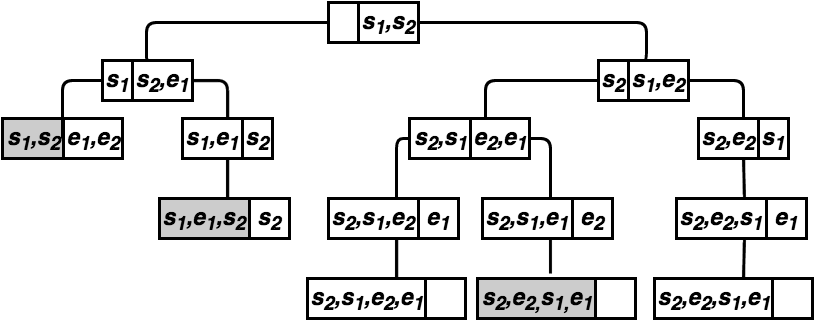
\includegraphics[width=0.75\columnwidth]{fig/bAndb.png}
	\vspace{-0mm}\caption{Illustration of \cref{algo:can_schedule}} \vspace{-2mm} \label{fig:bAndb}
\end{figure}\vspace{-0mm}

\vspace{-2mm}
\begin{algorithm}
	\caption{GetProfit($v, schedule, startTime$)}
	\label{algo:get_profit}
	\begin{algorithmic}[1]
		\REQUIRE \emph{schedule} is an ordered list of pick-up/drop-off points of driver $v$ and \emph{startTime} is the current time.
		\ENSURE the $profit$ of performing the input $schedule$ at time $startTime$. If $schedule$ is not valid it returns $-\infty$
		\STATE $time \leftarrow startTime$
		\STATE $loc \leftarrow v.$loc\label{ln:loc}
		\STATE $distance \leftarrow 0$
		\FOR{$p$ \textbf{in} $schedule$}
		\STATE $trip \leftarrow$ ShortestPath($loc, p$.loc)
		\STATE $distance \pluseq$ Distance($trip$)
		\STATE $time \pluseq$ TravelTime($trip$)
		\IF{$p$.type $==$ pick-up point}
		\IF{$time > p$.req.req\_time $ + $ p.req.w}\label{ln:mwt}
		\RETURN $-\infty$
		\ENDIF
		\STATE $pickUp[p$.req$]\leftarrow distance$
		\ENDIF
		\IF{$p$.type $ == $ drop-off point}
		\STATE $\Delta d \leftarrow distance - pickUp[p$.req$]$
		\IF{$\Delta d > p$.req.$\epsilon \times p$.req.sp}\label{ln:mad}
		\RETURN $-\infty$
		\ENDIF
		\STATE $fare \pluseq p$.req.f($\Delta d$) $\times$ F($p$.req.sp)\label{ln:delta}
		\STATE $cost \leftarrow v$.g($distance$)\label{ln:dprof}
		\ENDIF
		\STATE $loc \leftarrow p.loc$
		\ENDFOR
		\STATE $profit \leftarrow fare - cost$
		\RETURN $profit$
	\end{algorithmic} 
\end{algorithm}

\cref{algo:get_profit} computes the profit driver $v$ can generate by completing $schedule$ at $startTime$. Each driver $v$ runs this algorithm locally, and hence, $v.loc$ (line~\ref{ln:loc}) and $v.g$ (line~\ref{ln:dprof}) refer to $v$'s current location and profile, respectively. Also, for any node $p$ in the schedule, $p$.req and $p$.req.sp refer to the corresponding request of node $p$ and the shortest path for that request, respectively. \cref{algo:get_profit} iterates through the nodes in \textit{schedule} one by one keeping track of the added $time$ and $distance$. Each node is either a pick-up node or a drop-off node. For pick-up nodes, the algorithm checks if the maximum wait time constraint is violated (line~\ref{ln:mwt}). For every drop-off node, the detour constraint is checked (line~\ref{ln:mad}). If the check is successful, the algorithm computes the actual travel distance for the request and determines the incurred detour (line~\ref{ln:delta}). After computing the detour, the algorithm computes the added fare and cost using \cref{eq:fare,eq:payment,eq:profit}. If the input \textit{schedule} is not valid, the algorithm returns $-\infty$ as the profit.

Once drivers submit their bids, the server selects the driver with the highest bid and assigns the new request to that driver.
%The drives cost (income) is determined similar to \cref{algo:get_profit}.

%\subsection{Payments in \fname}

%Once every driver submits his bid, the server selects the driver with the highest bid as the winner and allocates the new request to him. Assuming driver $v$ wins the auction with probability $p_v$, his expected compensation is: 

%\begin{equation*}
%E[comp_v] = p_v.Comp_v(win) + (1 - p_v).Comp_v(loose)
%\end{equation*}

%Where $Comp_v()$ gives the compensation driver $v$ receives for winning or loosing the auction. Intuitively, in the case of winning, $v$ gets compensated the same amount as $cost_v$ based on which he determined his bid and receives $\$0$ for loosing, i.e., $E[comp_v] = p_v.cost_v$. We call this payment model first-price, since the compensation the winner receives is only based on the highest bid.

%Earlier we mentioned that the human driver has no interaction with \fname with regard to computing and submitting a bid. However, depending on how the human driver customizes his profile $g()$, he can affect his $cost$ computation and consequently, the bid value~\footnote{Hereafter, when we say the driver increases/decreases his bid, we mean he does it indirectly by customizing his profile}. For example, assume $v_i$ is the winner of the auction with bid $b_i$ and the second highest bid is $b_j$. In theory, if $v_i$ changes his profile such that his bid becomes $b_i - \epsilon (\epsilon < b_i - b_j)$, he will still be the winner of the auction and has gets compensated $\$\epsilon$ more than when his bid was $b_i$. In practice, however, $v_i$ does not know the \textit{actual} value of any other driver's bid. Therefore, for every driver there is a trade-off between lowering the value of the bid and the probability of being the winner. To maximize his compensation, a rational driver makes his bid as close as possible to the \textit{expected} value of the second highest bid. The details of how each driver can compute this expected value is out of the scope of this paper and more details can be found in \cite{Vickery61}.

%In order to facilitate the bid computation process for workers, \fname adopts a payment model in which the drivers do not benefit from increasing/decreasing their cost and bid values. The compensation of the winner driver in \fname is computed as:

%\begin{equation*}
%comp_i = cost_i + (bid_i - bid_j)
%\end{equation*}

%\noindent Where $v_i$ is the driver with the highest bid and $v_j$ is the driver with the second highest bid. Since the compensation depends on not only the highest bid but also the second highest bid, we call it the second-price model. Following we first prove that with the second-price model, each driver can maximize his compensation by configuring their profiles such that it results in the \textit{minimum} cost that is economical for him to participate in the system. Next we show that in the second-price payment model, not only we get the same rider to driver assignments, but also the final revenue of \fname in both model remains the same.

%\begin{theorem}
%In the second-price payment model, a driver has no incentive to configure his profiles such that his resulting cost is either lower or higher than his minimum cost.
%\end{theorem}

%\begin{theorem}
%Both the first-price and second-price payment model result in the same rider to driver assignment and generate the same revenue.
%\end{theorem}
%\section{Optimization}
Optimization ideas:
\begin{itemize}
	\item Adaptive grid index or hierarchy index
	\item Clever way of shortest path computation
	\item batch process trip request
\end{itemize}

Other ideas we have discussed:
\begin{itemize}
\item index sampling: use some sampling method to only send new requests to \emph{some} drivers.
\item index filtering: use a spatial index and send new request to drivers in the vicinity of the pickup location.
\item time threshold: wait for a certain amount of time and select the winning bid from bids received within that time. 
\item count threshold: once a certain number of bids are received, select the winning bid from them.
\end{itemize}
\section{Experiments}

\subsection{Dataset}
Dataset and experiment desig.

\subsection{Experiment Setup}

\subsubsection{Algorithms}
We compared the results of our framework (\textbf{APART}) with two other approaches; \textbf{SP} (i.e., Shortest Path) and \textbf{NN} (i.e., Nearest Neighbor).

Our implementation of SP is based on the algorithms in \cite{Huang14}. The only advantage of \cite{Huang14} over \cite{Ma13} is the the former considers reordering of the schedule while the latter does not. Although it is shown the performance increase of reordering requests is minimal, since we consider request reordering in APART, we decided to base the SP implementation on algorithms in \cite{Huang14} to make the comparison as fair as possible.

Also, the NN algorithm is implemented based on the current approach adopted by major ridesharing platforms such as Uber. The NN approach, finds the first nearest driver to the pick-up location of a new request. If the driver is able to fit the new request in its schedule without violating any constraints, he accepts the request. Otherwise the request is rejected and the algorithm tries to assign the request to the next nearest driver. This continues until a driver accepts the request of every driver rejects it in which case the request is dropped.

As a result, we are comparing the performance of APART with state-of-the-art approaches from both academia (SP) and industry (NN).

In the first set of experiments, we use the pricing model explained in \cref{subsec:pricing} and compare the three approaches. In ...... we utilize the pricing model introduced in \cite{Ma15} for both APART and SP. In the pricing model of \cite{Ma15}, there is no concept of \textit{revenue} similar to what we introduces in \cref{subsec:pricing}. Therefore, in order to compare the generated revenue, we assume each driver has to pay 20\% of what they make as the server's share.

\subsubsection{Configurations and Measures}
In our experiments we measure three different metrics by varying different parameters of the system. We measure (1) service rate as the percentage of requests that were completed, (2) the revenue of the system and (3) the response time for matching a request with a driver. Also, \cref{tab:params} shows the different values we used for various parameters to evaluate our framework (default values are shown in \textbf{bold}).

\TODO{mohammad}{Write default values for rider and driver profiles}

\begin{table}
\begin{center}
\begin{tabular}{|c|c|}
	\hline
	Parameter & Values \\
	\hline \hline
	Max Wait Time & 3min, \textbf{6min}, 9min, 12min, 15min, 20min \\ 
	\hline
	\# of Drivers & 1000, 2000, \textbf{5000},  10000, 20000\\ 
	\hline
	Max Passengers & 2, 3, \textbf{4}, 5, 6 \\
	\hline
	Max Allowed Detour & 25\%, \textbf{50\%}, 75\%, 100\%\\
	\hline
\end{tabular}
\caption{Parameters for Algorithm Comparison}
\label{tab:params}
\end{center}
\end{table}

\subsection{Algorithm Comparison}
In this section, we evaluate the performance of the three approaches by varying one of the parameters based on \cref{tab:params} while other parameters have their default values. We show how the algorithms compare to each other with regard to service rate, generated revenue and response time.

\subsubsection{Service Rate}
In the first set of experiments we compare the service rate of the three approaches. As shown in \cref{fig:sr}, all algorithms generate high service rates when the constraints are loosened or there is high resource availability. However, under tight constraints or limited resources, APART outperform the other two approaches by up to 20\%. To better explain the reason why APART has a higher service rate, we use the notion of \textit{eligible drivers} defined in \cref{subsec:dispatch}. \TODO{mohammad}{add a chart that shows the percentage of requests where in APART there are more eligible drivers}.

\begin{figure}[h]
    \centering
    \subfigure[\small{Maximum Wait Time}]{
        \label{fig:mwt_sr}
        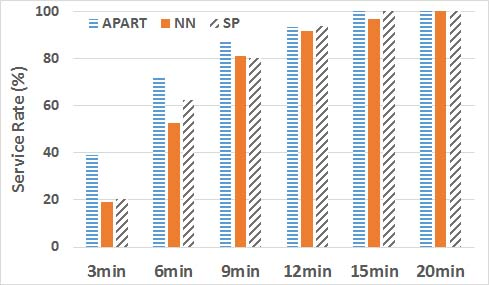
\includegraphics[width = 0.45\columnwidth]{fig/mwt_sr.jpg}
    }
    \subfigure[\small{Number of Drivers}]{
        \label{fig:nd_sr}
        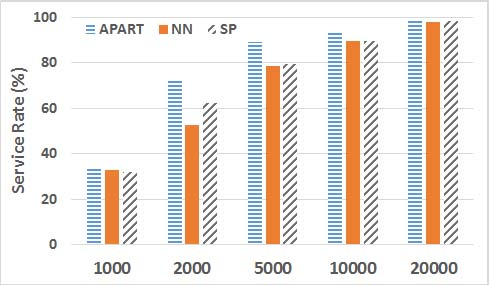
\includegraphics[width = 0.45\columnwidth]{fig/nd_sr.jpg}
    }
    \subfigure[\small{Maximum Passengers}]{
        \label{fig:mp_sr}
        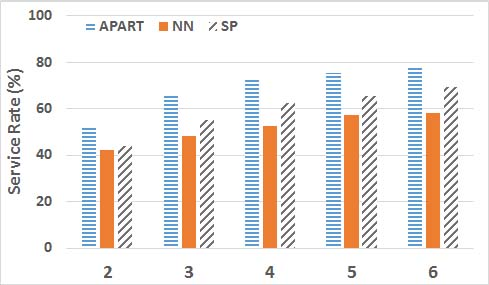
\includegraphics[width = 0.45\columnwidth]{fig/mp_sr.jpg}
    }
    \subfigure[\small{Maximum Allowed Detour}]{
        \label{fig:mad_sr}
        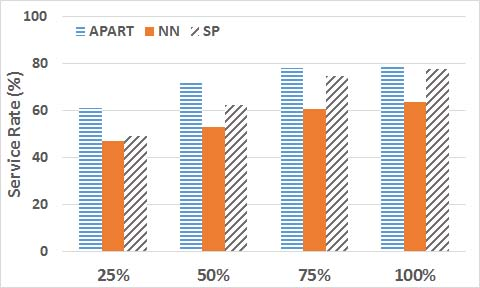
\includegraphics[width = 0.45\columnwidth]{fig/mad_sr.jpg}
    }
    \vspace{-0.15in}
    \caption{Comparing Service Rate of the Algorithms}
    \label{fig:sr}
\end{figure}

\subsubsection{Revenue}
As mentioned, the main objective of APART is to maximize the ridesharing platform's revenue. In these set of experiments, we compare the generated revenue of each algorithm. In these experiments we applied the pricing model explained in \TODO{mohammad}{ref to correct section} and used for the riders and drivers, used profiles similar to the ones in \TODO{mohammad}{ref to sample rider profiles} and \TODO{mohammad}{ref to sample driver profile} respectively. Here, we want to evaluate the effect of varying the parameters in \cref{tab:params} on the overall revenue and compare different algorithms. Later in \cref{subsec:pricingexp} we will apply different pricing models to the algorithms and compare revenue under different pricing models as well.

\begin{figure}[h]
    \centering
    \subfigure[\small{Maximum Wait Time}]{
        \label{fig:mwt_rev}
        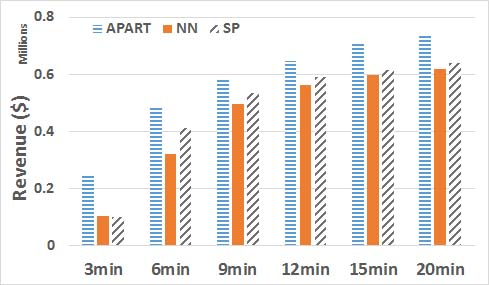
\includegraphics[width = 0.45\columnwidth]{fig/mwt_rev.jpg}
    }
    \subfigure[\small{Number of Drivers}]{
        \label{fig:nd_rev}
        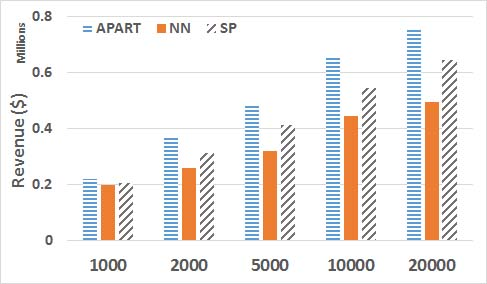
\includegraphics[width = 0.45\columnwidth]{fig/nd_rev.jpg}
    }
    \subfigure[\small{Maximum Passengers}]{
        \label{fig:mp_rev}
        \includegraphics[width = 0.45\columnwidth]{fig/mp_rev.jpg}
    }
    \subfigure[\small{Maximum Allowed Detour}]{
        \label{fig:mad_rev}
        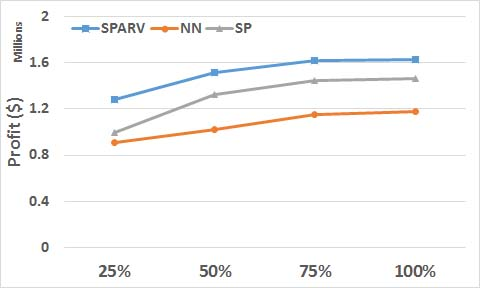
\includegraphics[width = 0.45\columnwidth]{fig/mad_rev.jpg}
    }
    \vspace{-0.15in}
    \caption{Comparing Revenue of the Algorithms}
    \label{fig:rev}
\end{figure}

As it can be seen in \cref{fig:rev} regardless of the values of different parameters, APART generates more revenue than any other approach. When we compare the results in \cref{fig:rev} with the ones in \cref{fig:sr}, even under configurations where all algorithms have the same service rate, APART manages to generate at least 10\% more revenue. The main reason for higher revenue is that APART is designed to make a \textit{Price-aware} assignment, i.e., assign the request to a driver that generates the most profit. Of course, as explained in \TODO{mohammad}{ref to pricing model section}, the pricing models that are used in APART are designed such that the higher profits are not gained by scamming the riders. On the other hand, as it was explained earlier, the SP and NN algorithm were not designed to maximize revenue. An interesting observation in \cref{fig:nd_ref} is that as more drivers are added, the profit decreases even though the service rate increases (\cref{fig:nd_sr}). The NN algorithm gives priority to drivers that are closer to the pick-up location of a request. As long as the driver is able to fit the request in its current schedule without violating the wait time and maximum detour constraints of any request, the request will be assigned to him. This means under certain conditions the sum of discounts other riders will receive can potentially be higher than the final fare of the new request and hence, the system will end up loosing money.

\subsubsection{Response Time}

Similar to \cite{Ma13,Huang14}, APART processes the requests, one request at a time once a request is submitted. In order to evaluate the scalability of our framework, our next set of experiments evaluate the response time of processing a single request. To count for the communication cost of these algorithms, for every message transfer, we add the communication cost as the \textit{message size} divided by a transmission rate of 1Mbit/sec (this is even less than the average speed of a 3G cellular network). \cref{fig:rp} compares the response time of the algorithms under different configurations.

\begin{figure}[h]
    \centering
    \subfigure[\small{Maximum Wait Time}]{
        \label{fig:mwt_rp}
        \includegraphics[width = 0.45\columnwidth]{fig/mwt_rp.jpg}
    }
    \subfigure[\small{Number of Drivers}]{
        \label{fig:nd_rp}
        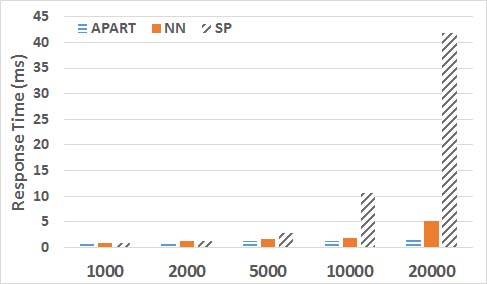
\includegraphics[width = 0.45\columnwidth]{fig/nd_rp.jpg}
    }
    \subfigure[\small{Maximum Passengers}]{
        \label{fig:mp_rp}
        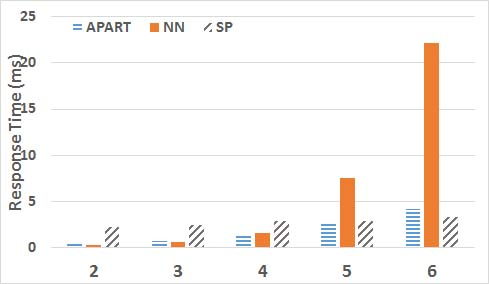
\includegraphics[width = 0.45\columnwidth]{fig/mp_rp.jpg}
    }
    \subfigure[\small{Maximum Allowed Detour}]{
        \label{fig:mad_rp}
        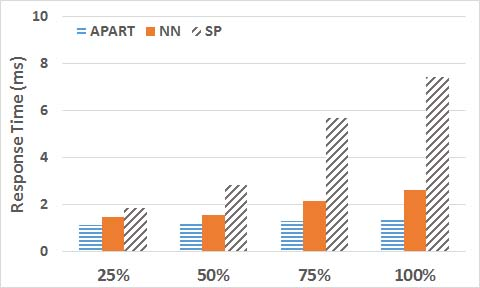
\includegraphics[width = 0.45\columnwidth]{fig/mad_rp.jpg}
    }
    \vspace{-0.15in}
    \caption{Comparing Revenue of the Algorithms}
    \label{fig:rp}
\end{figure}

In \cref{fig:mwt_rp}, the response time increases as more wait time is allowed. This is expected as more wait time, allows drivers to schedule more requests simultaneously which makes the scheduling more time consuming. However, all approaches manage to keep the response time less than 3ms which is acceptable for a real-time framework. However, in \cref{fig:nd_rp}, when more drivers are added, the scalability of SP suffers as it has to perform scheduling for a larger number of vehicles. On the other hand, due to the distributed nature of APART's auction-based approach, each driver does scheduling for itself and adding drivers does not affect the overall response time of APART as much. In \cref{fig:mp_rd} we notice that although APART's response time does not go beyond 2ms, SP handles the increase in maximum passengers better due to the Kinetic Tree structure implementation \cite{Huang14}. The reason for NN's poor performance in \cref{fig:mp_rp} is that it has to \textit{sequentially} perform a computation heavy scheduling, for possibly multiple drivers.

\subsection{Comparing Pricing Models}
\label{subsec:pricingexp}

\section{Related Work}
%In the following, we first review the related work regarding static ridesharing, then discuss real-time ridesharing. Pricing scheme and task assignment and scheduing in spatial crowdsouring.

% offline ridesharing
There are mainly two categories of ridesharing, i.e., static and dyanmic ridesharing. Most existing studies~\cite{FuruhataTRB13, Santi14, CiciUbicom14} belong to static ridesharing, where all riderS and drives are knownn in priori, and thus trips are prearranged. Furuhata et al.~\cite{FuruhataTRB13} provoides a compresensive suvery of the different types of ride sharing regarding their formulations, optimizations and key computations challenges. Santi et al.~\cite{Santi14} proposed a graph-based approach to quantify the potential of ridesharing using NewYork taxi data, and Cici et al.~\cite{CiciUbicom14} evaluated the potential of carpooling using four cities' mobile dataset. In addition, ridesharing problem can be treated as a special class of the dial-a-ride problem (DARP)~\cite{Cordeau07}, or dynamic vehicle routing problem (VRP)~\cite{LiSstd15} in operational research, which is proven to be NP-hard. All these studies assume that the rider and drivers status are know in advance, and hence can afford high computation cost, which is not the case in real-time ridesharing.

% real-time ridesharing
With the emergence of many ridesahring mobile applications (e.g., Uber and Lyft), real-time ridesharing~\cite{Ma13, Ma15, Huang14,OtaBigdata15, CiciGis15, CaoMDM15, PelzerITS15} attracts more research interest recently. Ma et al.~\cite{Ma13, Ma15} proposed a ridesharing dispatch system named ``T-share" to serve the rider request on-the-fly with the objective of reducing driver's total travel distance. Their work focus on maintaining a spatial-temporal indexing to retrieve the candidate drivers. On the other hand, Huang~\cite{Huang14} proposed a kinect tree scheduling algorithm to dynamically match trip request to drivers with minimum incurred travel distance. Ota et al.~\cite{OtaBigdata15} introduced a data-driven simuation framework that enables the analysis of ride-sharing by using NY taxi dataset. Santos et. al~\cite{SantosIjcai13} propose a ride sharing system to maximize the number of matched request. The majority of these studies aim to minimize the total travel distance of drivers, however, we show that this does not necessarily mean shorter travel distance for the riders. Compared with these work, we discuss the conflicting interest between riders, drivers and platform providers. We propose a general and flexible pricing scheme and  our objective is to maximize the total profit of platform. We show that by maximizing the overall profit, our framework achieves higher service rate and quality.  Finally, We introduced a decentralized auction-based framework to support scalable and real-time scheduling, which differs existing centralized scheduling framework. 
%Because of this decentralized framework, the kinect tree scheduling algorithm proposed in Huang~\cite{Huang14} can be easily integrated into APART to purse further efficiency. \dingedit{Do we need this last sentence?}

% pricing scheme
Pricing mechanisms in realtime ridesharing have also been studied in~\cite{KamarIJCAI09,KleinerIJCAI11, ZhaoAAMAS14}. Their main focus is to adapt the well-known VCG mechanism~\cite{Nisan07} for truthful bidding, while addressing the specific challenges such as computational issues, incentive compatibility~\cite{KamarIJCAI09, KleinerIJCAI11} and deficit control~\cite{ZhaoAAMAS14}. These studies are orthogonal to our paper, and can be integrated into our framework APART when we compute the bid of each candidate driver. 

% spatial crowdsourcing
Our work is also related to the task assignment and scheduling problem in spatial crowdsourcing~\cite{KazemiGis12, DengGis13, DengGis15}. Spatial crowdsourcing is a platform, whic enables a requester to comission workers to physically travel to some specified locations to perform a set of spatial tasks. For example, Kazemi et. al~\cite{KazemiGis12} formuated task assignment in spatial crowdsourcing as a min-cost max-flow problem, Deng et. al studied both task scheduling problem for one single worker~\cite{DengGis13} and multiple workers~\cite{DengGis15}. Different with spatial crowdsourcing, in real-time ridesharing, each rider request consists of both pickup and dropoff locations. In addition, their assignment and scheduling are processed in a batch fashion (e.g., batching tasks and workers every 10 minutes), whereas each rider requst in realtime ridesharing must be processed in a short amount of time.

\section{Conclusion}

\section*{Acknowledgement}
This research has been funded in in part by NSF grants IIS-1320149 and CNS-1461963, METRANS Transportation Center under grants from Caltrans (DTRT12-G-UTC57), the USC Integrated Media Systems Center, and unrestricted cash gifts from Google, Northrop Grumman and Oracle. Any opinions, findings and conclusions or recommendations expressed in this material are those of the authors and do not necessarily reflect the views of any of the sponsors.

\begin{scriptsize}
%\begin{footnotesize}
\bibliographystyle{IEEEtran}
\bibliography{sharing}
%\end{footnotesize}
\end{scriptsize}

\end{document}
